\chapter{Modeling And Evaluation}

\section{Select Modeling Tecnique}

\subsection{Modeling Technique for Classification}
% Document the modeling technique that you’ll be using
Random Forest Tree: Random forest is an ensemble learning method for classification, regression and other tasks that operate by constructing a multitude of decision trees at training time and outputting the class that is the mode of the classes (classification) or mean prediction (regression) of the individual trees. Random forest is known for its accuracy and robustness to noise and outliers.

Naive Bayes: Naive Bayes is a probabilistic algorithm that is based on Bayes’ theorem. Naive Bayes is used for classification problems and is known for its simplicity and speed.

Decision Tree: A decision tree is a supervised learning algorithm that is used for classification and regression modeling. It is a method used for predictive modeling, so these trees are used to either classify data or predict what will come next. Decision trees in machine learning can either be classification trees or regression trees. 

\subsection{Modeling Technique for Clustering}

Bisecting K-means: Bisecting K-means is a hierarchical clustering algorithm that recursively bisects clusters until the desired number of clusters is reached. The algorithm starts with all data points in one cluster and then splits the cluster into two smaller clusters. The splitting is done by running K-means on the larger cluster and splitting it into two smaller clusters based on the K-means output. The process is repeated until the desired number of clusters is reached.

K-means: K-means is a clustering algorithm that partitions n observations into k clusters in which each observation belongs to the cluster with the nearest mean. The algorithm starts by randomly selecting k initial centroids. Each observation is then assigned to the nearest centroid. The mean of each cluster is then calculated and used as the new centroid. This process is repeated until the centroids no longer change or a maximum number of iterations is reached.

Gaussion Mixture: Gaussian Mixture Model (GMM) is a probabilistic model that assumes that the data is generated from a mixture of several Gaussian distributions with unknown parameters. The algorithm starts by randomly initializing the parameters of the Gaussian distributions. The expectation-maximization (EM) algorithm is then used to estimate the parameters of the Gaussian distributions. The EM algorithm iteratively estimates the parameters of the Gaussian distributions until convergence. 

\subsection{Modeling Assumptions}
% Record any assumptions about the data that are necessary for the modeling techniques
Random Forest Tree: Random forest assumes that the data is independent and identically distributed (i.i.d.) and that there are no missing values in the data.

Naive Bayes: Naive Bayes assumes that the features are independent of each other and that there are no missing values in the data.

Decision Tree: Decision tree is a non-statistical approach that makes no assumptions of the training data or prediction residuals; e.g., no distributional, independence, or constant variance assumptions.

Bisecting K-means: Bisecting K-means makes no assumptions about the underlying data distribution 

K-means:The variance of the distribution of each attribute (variable) is spherical and all variables have the same variance.

Gaussian mixture models: Gaussian mixture models (GMMs) are a probabilistic model that assumes all the data points are generated from a mixture of a finite number of Gaussian distributions with unknown parameters

\section{Build Model And Evaluation}  

We used the \textit{org.apache.spark.ml} library for the training process. There also employed 5-fold cross-validation to train the model and select the best model for evaluation.
\subsection{Random Forest Tree}

After Modeling the result of Confusion Matrix~\ref*{cmRFT} and evaluation table~\ref*{tableRFT} list here.


\begin{table}[H]  \centering  
    \begin{tabular}{@{}lllll@{}}
    \toprule
    \multicolumn{5}{c}{Random Forest Tree}                 \\ \midrule
    \multicolumn{5}{l}{Accuracy: 0.9775641025641025}       \\\midrule
                 & precision & recall & f1-score & FPR \\
    0.0         & 0.97      & 0.99   & 0.98     & 0.01      \\ 
    1.0          & 0.98      & 0.93   & 0.96     & 0.00     \\
    2.0       & 0.97      & 1.00   & 0.98     & 0.01     \\
    
    Weighted precision    & \multicolumn{4}{c}{0.977800279509976}         \\
    Weighted recall    & \multicolumn{4}{c}{0.977564102564102}          \\
    Weighted F1 score    & \multicolumn{4}{c}{0.977369021913490}        \\
    Weighted false positive rate & \multicolumn{4}{c}{0.011880522633986}         \\ \bottomrule
    \end{tabular}
    \caption{Classification Report of Random Forest}
    \label{tableRFT}
\end{table}





\begin{figure}[H]
    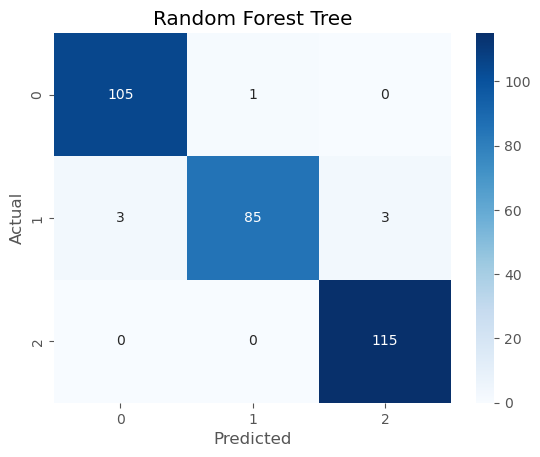
\includegraphics[scale=0.7]{imgs/rft}
    \centering
    \caption{Confusion Matrix of Random Forest Tree}
    \label{cmRFT}
\end{figure}


\subsection{Naive Bayes}

As for the Naive Bayes, the result of Confusion Matrix~\ref*{cmnb} and evaluation table~\ref*{tablenb} list here.


\begin{table}[H]\centering
    \begin{tabular}{@{}lllll@{}}
    \toprule
    \multicolumn{5}{c}{Naive Bayes}                 \\ \midrule
    \multicolumn{5}{l}{Accuracy: 0.7852564102564102}       \\\midrule
                 & precision & recall & f1-score & FPR \\
    0.0         & 0.78      & 0.95   & 0.84     & 0.16      \\ 
    1.0          & 0.70      & 0.45   & 0.55     & 0.07     \\
    2.0       & 0.85      & 0.89   & 0.87     & 0.08     \\
    
    Weighted precision    & \multicolumn{4}{c}{0.7786264164368255}         \\
    Weighted recall    & \multicolumn{4}{c}{0.7852564102564104}          \\
    Weighted F1 score    & \multicolumn{4}{c}{0.7695695968516545}        \\
    Weighted false positive rate & \multicolumn{4}{c}{0.1086680781804235}  \\ \bottomrule
    \end{tabular}
    \caption{Classification Report of Naive Bayes}
    \label{tablenb}
    \end{table}

\begin{figure}[H]
    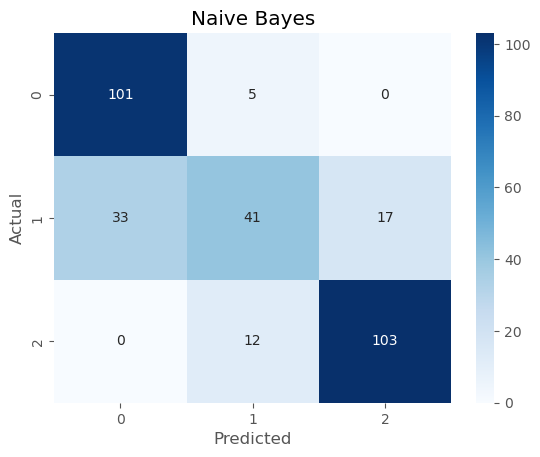
\includegraphics[scale=0.7]{imgs/nb}
    \centering
    \caption{Confusion Matrix of Naive Bayes}
    \label{cmnb}
\end{figure}

\subsection{Decision Tree} 

The DecisionTreeClassifier is a class in the sklearn.tree module of the Python Scikit-learn library. It is used to create a decision tree classifier which is a predictive model that can be used for both classification and regression problems. The criterion parameter specifies the function to measure the quality of a split. In this case, we use the supported criteria is “gini” for the Gini impurity.
Confusion Matrix~\ref{cmdt} and Classification Report of Decision Tree~\ref{tabledt}.
\begin{table}[H]\centering
    \begin{tabular}{@{}lllll@{}}
    \toprule
    \multicolumn{5}{c}{Decision Tree}                 \\ \midrule
    \multicolumn{5}{l}{Accuracy: 0.8269230769230769}       \\\midrule
                 & precision & recall & f1-score & FPR \\
    0.0         & 0.84      & 0.90   & 0.82     & 0.08      \\ 
    1.0          & 0.71      & 0.67   & 0.69     & 0.10     \\
    2.0       & 0.89      & 0.87   & 0.88     & 0.06     \\
    
    Weighted precision    & \multicolumn{4}{c}{0.8248610604716251}         \\
    Weighted recall    & \multicolumn{4}{c}{0.8269230769230769}          \\
    Weighted F1 score    & \multicolumn{4}{c}{0.8252391066535802}        \\
    Weighted false positive rate & \multicolumn{4}{c}{0.0838127083514056}  \\ \bottomrule
    \end{tabular}
    \caption{Classification Report of Decision Tree}
    \label{tabledt}
    \end{table}

    \begin{figure}[H]
        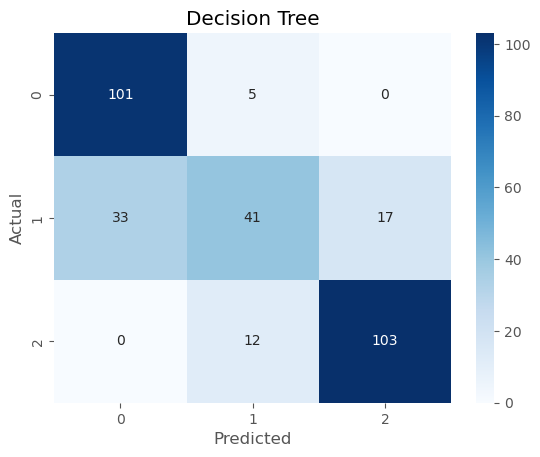
\includegraphics[scale=0.7]{imgs/dc}
        \centering
        \caption{Confusion Matrix of Decision Tree}
        \label{cmdt}
    \end{figure}

\subsection{Clustering Task}

The Silhouette method is a way to evaluate the quality of clustering. It measures how similar an object is to its own cluster compared to other clusters. The Silhouette score ranges from -1 to 1. A score of 1 indicates that the object is well matched to its own cluster and poorly matched to neighboring clusters.
the table\ref{cluster} show the performance of each algorithms.
\begin{table}[]
    \begin{tabular}{ll}
    \hline
    \multicolumn{2}{c}{Cluster Task}                                                     \\ \hline
                        & \multicolumn{1}{c}{Silhouette with squared euclidean distance} \\
    K means             & 0.2185969767629818                                             \\
    Gaussian Mixture    & 0.2139769508957303                                             \\
    Biselecting K-means & 0.3698272179197341     \\ \bottomrule
    \end{tabular}
    \caption{Evaluation of Cluster}
    \label{cluster}    
    \end{table}